%\iffalse
\begin{frame}{Questions to Keep in Mind}

\begin{itemize}
\item <+-> What problem are we solving?
\item <+-> Why do we want to solve it?
\item <+-> What are some notable results in our work?
%\item <+-> ``The Surprising Power of Constant Depth Algebraic Proofs'' has 37 pages and on ECCC
%\item <+-> I really want to thank the original speaker 
\end{itemize}

\end{frame}
%\fi

%%thinking of n-body problem, not just interested in d = 3.
%% atucal force vector, simplify to sum of scalars


%\begin{frame}
%\begin{itemize}
%  \item <+-> Given a matrix $A$, you want to do some tasks
%\end{itemize}
%\end{frame}

\begin{frame}{Fast Algorithms on Geometric Graphs ($K$-Graphs)}

\begin{itemize}
  \item <+-> Our problem: find fast algorithms on geometric graphs
    (complete graphs from $n$ points in $d$ dimensions).
  \item <+-> There are {\color{red}$n^2$} edges in the graph, but input
    is size {\color{darkgreen}$nd$}.
  \item <+-> When $d = o(n)$, we can hope for $o(n^2)$ algorithms.
\end{itemize}
\end{frame}
\begin{frame}{Fast Algorithms on Geometric Graphs ($K$-Graphs)}
  We consider a special class of these graphs, $K$-graphs.
  \begin{itemize}
  \item <+-> What's a $K$-graph?
  \item <+-> What algorithms are we considering?
\end{itemize}
\end{frame}
\begin{frame}{What is a $K$-graph?}
  \begin{itemize}
  \item <+-> Let $K:\mathbb{R}^d \times \mathbb{R}^d \rightarrow
    \mathbb{R}^{\geq 0}$.
  \item <+-> The \textbf{K- graph} of a set of $n$ points $x_1, \ldots
    x_n \in \mathbb{R}^d$ is a complete graph of $n$ nodes. The edge
    weight between node $i$ and $j$ is $K(x_i, x_j)$.
%\item <+-> ``The Surprising Power of Constant Depth Algebraic Proofs'' has 37 pages and on ECCC
%\item <+-> I really want to thank the original speaker 
\end{itemize}
\end{frame}
% \begin{center}
% 
% 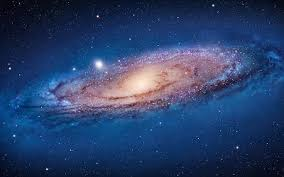
\includegraphics[width=.9\textwidth]{figs/galaxy}
% \end{center}
% 
% \end{frame}


\begin{frame}{Examples of $K$ and $K-graphs$}
\begin{itemize}
  \item <+-> In our talk, we restrict our attention to functions $K$ where
    $K(x,y) = f(\|x-y\|_2)$.
  \item <+-> \textbf{Example:} Let $K(x,y) = \|x-y\|_2$. Then the $K$-graph
    of $x_1, \ldots x_n$ is the complete graph of $n$ vertices whose
    edge lengths are the Euclidean distance between points.
  \begin{center}
  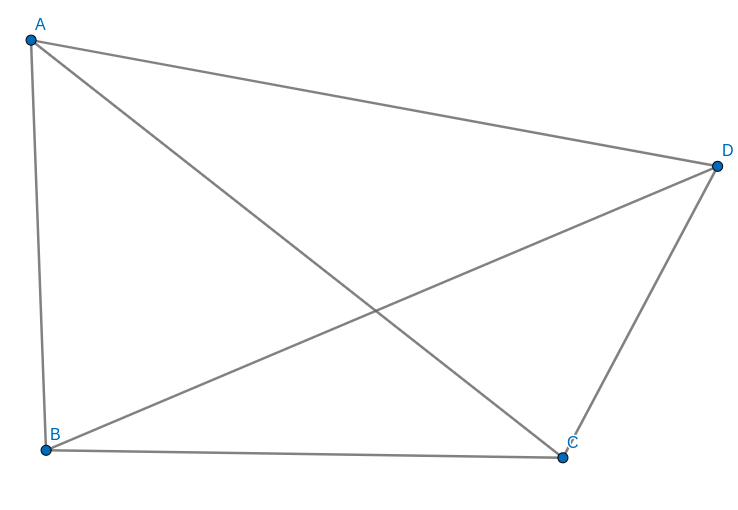
\includegraphics[width=.4\textwidth]{figs/complete_euclidean_graph}
  \end{center}
  \item <+-> \textbf{Example:} Let $K(x,y) = \frac{1}{\|x-y\|_2^2}$. Then the $K$-graph
    of $x_1, \ldots x_n$ is the complete graph of $n$ vertices whose
    edge lengths are the inverse squared Euclidean distance between points.
\end{itemize}

% \begin{tikzpicture}
%   \draw (0,0) -- (2, 0) -- (1, 1);
%   \draw[black, very thick] (0, 0) -- ++ (0, 4.25);
% % \node<1-> (z) at (-1,5) {{\color{white} . }};
% % \node<1-> (z) at (10,5) {{\color{white} . }};
% % \node<1-> (z) at (-1,0) {{\color{white} . }};
% % \node<1-> (z) at (10,0) {{\color{white} . }};
% %     
% % \node<1-> [] (z) at ( 5,2.5 ) {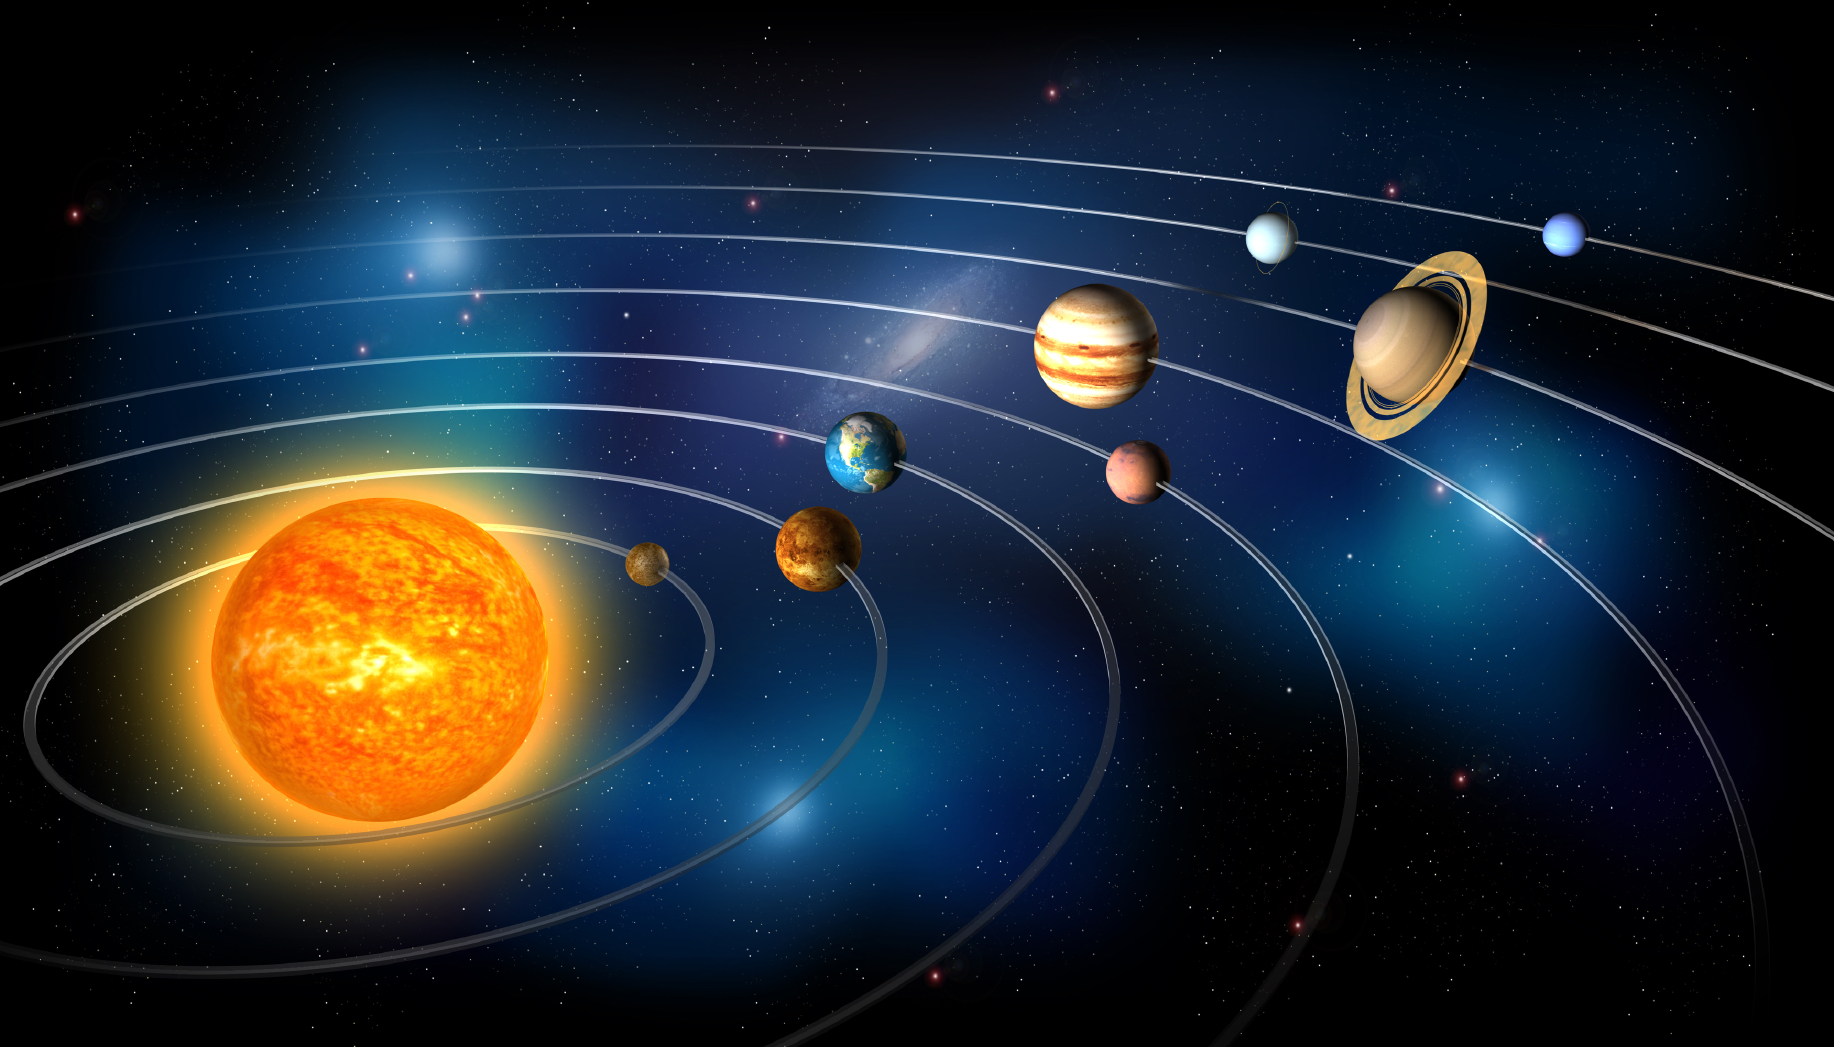
\includegraphics[height=5 cm]{./figs/solar_system}};
% \end{tikzpicture}
\end{frame}

%%%% Mercury, Venus, Earth, Mars, Jupiter, Saturn, Uranus, Neptune
\begin{frame}{Fast Algorithms on Geometric Graphs ($K$-Graphs)}
  We consider a special class of these graphs, $K$-graphs.
  \begin{itemize}
  \item What's a $K$-graph?
  \item What algorithms are we considering?
\end{itemize}
\end{frame}

 \begin{frame}
  \frametitle{What algorithms are we considering?}
   For what $\textbf{K}$ and $\textbf{d}$ does the $K-graph$ on $n$
   points in $d$ dimensions have fast algorithms approximating:
  \begin{itemize}
    \item <+-> The {\color{red}matrix vector multiplication problem}:
      Multiplying the $K$-graph's adjacency matrix or Laplacian matrix
      by any $n$ dimensional vector with high accuracy.
    \item <+-> The {\color{darkblue}spectral sparsifier problem}: Finding a
      spectral sparsifier to the $K$-graph.
    \item <+->  The {\color{darkgreen}Laplacian System Solver}:
      Approximate x (with high-accuracy) such that $Lx=b$ for given $b$.
      Here, $L$ is the Laplacian of the $K$-graph.
  \end{itemize}
 \end{frame}

 \begin{frame}
  \frametitle{What algorithms are we considering?}
   The {\color{red}matrix vector multiplication problem}:
   \begin{center}
     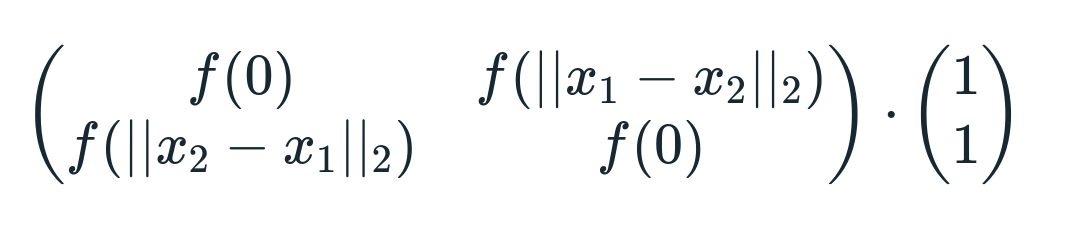
\includegraphics[width=1\textwidth]{figs/mv.png}
   \end{center}
 \end{frame}

 \begin{frame}
  \frametitle{What algorithms are we considering?}
    The {\color{darkblue}spectral sparsifier problem}:
    \begin{center}
     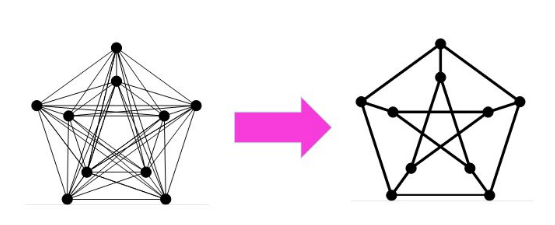
\includegraphics[width=1\textwidth]{figs/sparsifier.png}
   \end{center}
 \end{frame}

 \begin{frame}
  \frametitle{What algorithms are we considering?}
    The straightforward running time for these problems is
      $O(n^2)$. Our desired runtime is $n^{1+o(1)}$, when $d$ is $O(\log
      n)$. Here, dependence on our approximation factor is hidden.
  \end{frame}
